\documentclass{article}
\usepackage{LectureNotes}

\setstretch{1.2}

\begin{comment}
\geometry{
    textheight=9in,
    textwidth=5.5in,
    top=1in,
    headheight=12pt,
    headsep=25pt,
    footskip=30pt
}
\end{comment}


\geometry
{
    a4paper,
    total={170mm,257mm},
    left=20mm,
    top=20mm,
}


% ------------------------------------------------------------------------------

\begin{document}

% ------------------------------------------------------------------------------
% Cover Page and ToC
% ------------------------------------------------------------------------------

\title{ \normalsize \textsc{}
		\\ [2.0cm]
		\HRule{1.5pt} \\
		\LARGE \textbf{\uppercase{40.002 Optimization}
		\HRule{2.0pt} \\ [0.6cm] \LARGE{An Introduction to Optimization} \vspace*{10\baselineskip}}
		}
\date{\today}
\author{\textbf{Michael Hoon}}

\maketitle
\newpage

\tableofcontents
\newpage

% ------------------------------------------------------------------------------

\section{Introduction to Linear Programming}
An optimization problem is defined by:

\begin{itemize}
    \item \textbf{Decision variables}: elements under the control of the decision maker
    \item \textbf{A (single) objective function}: a function of the decision variables that we want to optimize, corresponding to a criterion for measuring maximize
    \item \textbf{Constraints}: restrictions that define which values of the decision variables are allowed.
\end{itemize}

\noindent We want to find the \textbf{minimum} or \textbf{maximum} of a function of one or many variables subject to a set of \textbf{constraints}:

\begin{align}
    & \min \; f(x_{1}, \dots x_n) \\ \nonumber
    & \ni(x_{1}, \dots x_n) \in \chi \subseteq \mathbb{R}^{n}
\end{align}

\noindent where the decision variables are vectors $x_{1}, \dots x_n$, the objective function is $f(x_{1}, \dots x_n)$ and the constraints are defined by the set $\chi \subseteq \mathbb{R}^{n}$. A vector $\mathbf{x}^{*}$ is called \textit{optimal}, or a \textit{solution} of the problem, if it has the \textbf{smallest objective value} among all vectors that satisfy the constraints. 

\subsection{Standard Form}
A linear program is a class of optimisation problem in which the objective and all constraint functions are \textbf{linear}. For a minimisation problem,

\begin{align}
    & \min \; \mathbf{c}^{\top} \mathbf{x} \\ \nonumber
    & \ni \mathbf{Ax} \geq \mathbf{b}, \; \text{and} \; \mathbf{x} \geq 0
\end{align}

\noindent and for maximisation problems,

\begin{align}
    & \max \; \mathbf{c}^{\top} \mathbf{x} \\ \nonumber
    & \ni \mathbf{Ax} \leq \mathbf{b}, \; \text{and} \; \mathbf{x} \geq 0
\end{align}

\noindent where the decision vector is $\mathbf{x}$ (n variables), linear objective function: $f(\mathbf{x}) = \mathbf{c}^{\top} \mathbf{x} = \sum_{i=1}^{n} c_i x_i $, and the linear constraints are $\chi = \{\mathbf{x} \in \mathbb{R}^{n}\mid \mathbf{Ax} \geq \mathbf{b}\}$ (m constraints) \footnote[1]{Note: vector inequalities are interpreted componentwise.}. Note that matrix $\mathbf{A}_{(m\times n)}$ is of $m \times n$ dimension. 

\subsubsection{Inequality Transformations}

We have matrix $\mathbf{A}$ given by:

\begin{equation*}
    \mathbf{A} = \begin{pmatrix}
        - & \mathbf{a_1}^{\top} & - \\ 
        \vdots & \vdots & \vdots \\ 
        - & \mathbf{a_m}^{\top} & -
    \end{pmatrix}
\end{equation*}

\begin{itemize}
    \item An equality constraint $\mathbf{a_i}^{\top} \mathbf{x} = b_i$ is equivalent to two equality constraints $\mathbf{a_i}^{\top} \mathbf{x} \leq b_i$ and $\mathbf{a_i}^{\top} \mathbf{x} \geq b_i$
    \item An inequality constraint $\mathbf{a_i}^{\top} \mathbf{x} \leq b_i$ is equivalent to the inequality constraint $-\mathbf{a_i}^{\top} \mathbf{x} \geq -b_i$ (Note the negatives applied to both sides of the inequality).
    \item Constraints such as $x_j \geq 0, \; x_j \leq 0$ can be expressed in the form $\mathbf{a_i}^{\top} \mathbf{x} \geq b_i$ by appropriately choosing $\mathbf{a}_i, \; b_i$.
\end{itemize}

\noindent Note that there is no simple analytic formula for the solution of a linear program, but there are a variety of effective methods for solving them, including Dantzig's simplex method, and the more recent interior-point methods. We cannot give the exact number of arithmetic operations required to solve a linear program, but we can establish rigorous bounds on the number of operations required to solve a linear program using an interior-point method (in practice, this is of the order $n^{2}m$, assuming $m \geq n$). 

\subsubsection{Terminology}

\begin{definition}
    We now introduce some terminology for geometric linear programming:
    \begin{itemize}
        \item A \textbf{linear function} $f : \mathbb{R}^{n} \to \mathbb{R}$ is a function of the form: \begin{equation*}
            f(x_{1}, \dots , x_n) = \sum_{i=1}^{n} a_i x_i, \quad a_i \in \mathbb{R}
        \end{equation*}
        \item A \textbf{hyperplane} in $\mathbb{R}^{n}$ is the set of points satisfying a single linear \textbf{equation}:
        \begin{equation*}
            a_{1}x_{1} + \dots + a_n x_n = b, \quad a_n \in \mathbb{R}
        \end{equation*}
        \item A \textbf{halfspace} in $\mathbb{R}^{n}$ is the set of points satisfying a single linear \textbf{constraint}: 
        \begin{equation*}
            a_{1}x_{1} + \dots + a_n x_n \geq b, \quad a_n, b \in \mathbb{R}
        \end{equation*}
        \noindent A halfspace is a \textbf{convex set}.
        \item An LP is \textbf{bounded} if there is some value $Z$ such that $\mathbf{c}^{\top}\mathbf{x} \leq Z$. 
        \item A \textbf{polyhedron} is a set that can be described by a finite number of halfspaces. A \textbf{polytope} is a \textbf{bounded} polyhedron. The polytope of an LP is \textbf{convex}, since it is the intersection of halfspaces (which are convex).
        \item An assignment of values to the decision variables is a \textbf{feasible solution} if it \textbf{satisfies all the constraints} (infeasible otherwise). The set of all feasible solutions is the \textbf{feasible region.}
        \item An \textbf{optimal solution} is a feasible solution that achieves the \textbf{best possible objective function value}. For a minimisation problem, $x^{*}$ is optimal \textbf{iff} $\mathbf{c}^{\top} \mathbf{x^{\top}} \leq \mathbf{c}^{\top} \mathbf{x}$ for all feasible $\mathbf{x}$. 
        \item We call $\mathbf{c}^{\top} x^{*}$ the \textbf{optimal objective value}. 
        \item $\forall K \in \mathbb{R}$ we can find a feasible solution $\mathbf{x}$ such that $\mathbf{c}^{\top}\mathbf{x} \leq K$, then the linear program in \textbf{minimisation} form has \textbf{unbounded} cost. The optimum cost is then $-\infty$. In this case, we can find a feasible $\mathbf{x}$ and direction $\mathbf{d}$ such that $\mathbf{x} + t \mathbf{d}$ is feasible $\forall t \geq 0$ and $\mathbf{c}^{\top}d < 0$.
    \end{itemize}    
\end{definition}

\noindent For every linear program, we know that one of the following cases must hold:

\begin{enumerate}
    \item The LP is infeasible. There is no value of $x$ that satisfies the constraints. 
    \item The LP has an optimal solution
    \item The LP is unbounded. 
\end{enumerate}

\noindent Mathematically, this follows from the fact that if the LP is \textbf{feasible and bounded}, then it is a closed and bounded subset of $\mathbb{R}^{n}$ and hence has a maximum point. 

\subsection{Geometric Definition}

In a simple two-dimensional space with the equation $x_{1} + x_{2} = z$, this function can be represented by a line. The decision variables are $x_{1}$ ad $x_{2}$, and this line represents all possible combinations of $x_{1}$ and $x_{2}$ that yield the same objective value $z$. \\ 

\noindent Each constraint is a linear inequality, which creates a boundary in the solution space. The feasible region is now the polygon formed by the intersection of all these constraint boundaries. \\

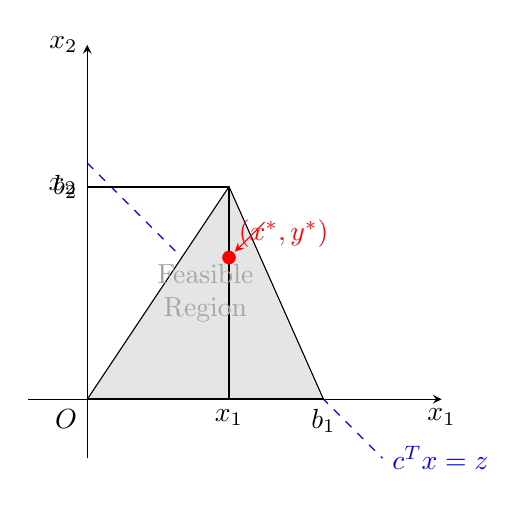
\begin{tikzpicture}[>=stealth, scale=1.5]
    % Objective function
    \draw[->] (-0.5,0) -- (3,0) node[below]{$x_1$};
    \draw[->] (0,-0.5) -- (0,3) node[left]{$x_2$};
    \draw[dashed, domain=0:2.5, variable=\x, blue] plot ({\x}, {2-\x}) node[right]{$c^Tx = z$};
  
    % Constraints
    \filldraw[fill=gray!20] (0,0) -- (2,0) -- (1.2,1.8) -- cycle;
    \draw[thick] (2,0) -- (0,0) node[below left]{$O$};
    \draw[thick] (1.2,1.8) -- (1.2,0) node[below]{$x_1$};
    \draw[thick] (1.2,1.8) -- (0,1.8) node[left]{$x_2$};
    
    % Labels
    \node[below] at (2,0) {$b_1$};
    \node[left] at (0,1.8) {$b_2$};
  
    % Optimal solution
    \filldraw[red] (1.2,1.2) circle (1.5pt) node[above right]{$(x^*,y^*)$};
    
    % Arrow to optimal solution
    \draw[->, red] (1.5,1.5) -- (1.25,1.25);
  
    % Feasible Region label
    \node[gray!70, align=center] at (1,0.9) {Feasible\\Region};
  \end{tikzpicture}

\noindent The feasible region is often convex, meaning that if points A and B are inside the region, the line segment connecting A and B are also inside the region. Some examples are shown below: \\

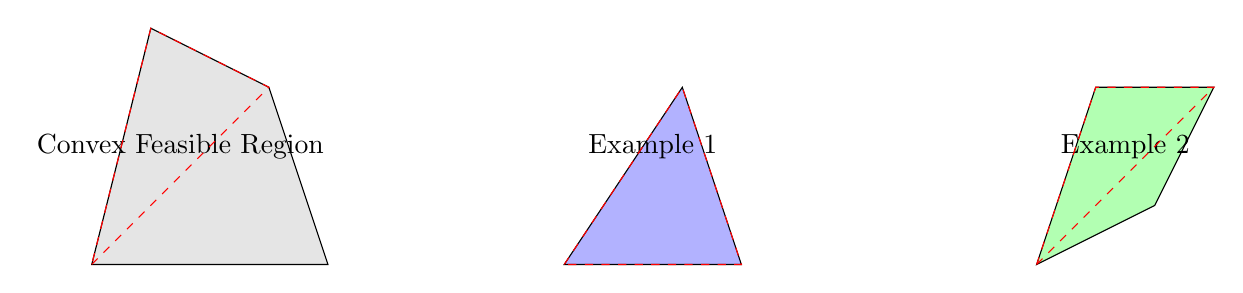
\begin{tikzpicture}[>=stealth, scale=1.5]
    % Convex Feasible Region
    \filldraw[fill=gray!20] (0,0) -- (2,0) -- (1.5,1.5) -- (0.5,2) -- cycle;
  
    % Convex Examples
    \filldraw[fill=blue!30, xshift=4cm] (0,0) -- (1.5,0) -- (1,1.5) -- cycle;
    \filldraw[fill=green!30, xshift=8cm] (0,0) -- (1,0.5) -- (1.5,1.5) -- (0.5,1.5) -- cycle;
  
    % Labels
    \node at (0.75,1) {Convex Feasible Region};
    \node at (4.75,1) {Example 1};
    \node at (8.75,1) {Example 2};
  
    % Convex Hulls
    \draw[dashed, red] (0,0) -- (1.5,1.5) -- (0.5,2) -- (0,0);
    \draw[dashed, red, xshift=4cm] (0,0) -- (1,1.5) -- (1.5,0) -- (0,0);
    \draw[dashed, red, xshift=8cm] (0,0) -- (1.5,1.5) -- (0.5,1.5) -- (0,0);
  \end{tikzpicture} \\


\subsection{Graphical Approach}

Solving the LP via a graphical approach involves drawing the halfspaces defined by the constraints, as well as the iso-lines defined by the optimisation problem. \\

\begin{figure}[H]
    \centering
    \includegraphics[width=0.5\textwidth]{Images/LP_Graphical.png}
    \caption{A linear Program in 2 dimensions}
    \label{fig:lpdiag}
\end{figure} 

\noindent After determining the bounded-ness of the LP problem, shade the feasible region (polytope) defined by the constraints. Points within this feasible region satisfy all constraints, and is a \textbf{convex polygon}. \\

\noindent Note that the feasible region for an LP may be \textit{empty, a single point, or infinite (unbounded)}. Our goal now is to find a point in the feasible region that optimises this objective. Since there are an infinite number of possible points within the polytope, we need to reduce this space. 

\begin{theorem}
    The maximum point for an LP is always achieved at one of the vertices of a polytope. In general, if there are $n$ dimensions (variables), a vertex may occur wherever $n$ (linearly independent) hyperplanes (i.e. constraints) intersect.
\end{theorem}

\noindent Recall in linear algebra that if you have $n$ linearly independent equations and $n$ variables, there is only one optimal solution (and if they are not linearly independent - you have infinitely many solutions). So in a system with $m$ constraints and $n$ variables, there are $\binom{m}{n} = O(m^{n})$ vertices. \\ 

\noindent Now, to determine which of the vertices gives the maximum objective value, we can substitute the variables into the objective function and compare the final values \footnote[2]{Note that at each vertex, if the iso-line falls within the polytope, then it is not a maximum.} 

\subsubsection{Geometric Intuition}
The objective function gives the optimisation direction, and the goal is to find the feasible point that is furthest in this direction. 

\subsection{Convexity}
When optimisation is concerned, we equate "convex" with "nice", and "non-convex" with "nasty". 

\subsubsection{Convex Sets}

\begin{theorem}
    The feasible region (Polytope) of an LP is \textbf{convex}. 
\end{theorem}

\noindent Intuitively, a subset $C\subseteq \mathbb{R}^{n}$ is convex if it is "filled in", meaning that it contains all line segments between its points (if you draw a line segment between two points of the region, the line segment itself must be in the region). 

\begin{figure}[H]
    \centering
    \includegraphics[width=0.7\textwidth]{Images/convexity.png}
    \caption{Examples of convex and non-convex sets}
    \label{fig:1-convex}
\end{figure} 

\noindent Mathematically, a set $\chi \subseteq \mathbb{R}^{n}$ is convex if 

\begin{equation*}
    \lambda \mathbf{x} + (1-\lambda)\mathbf{y} \in \chi, \; \forall \mathbf{x}, \mathbf{y} \in \chi, \; \forall \lambda \in [0,1]
\end{equation*}

As $\lambda$ ranges from 0 to 1, it traces out the line segment from $\mathbf{y}$ to $\mathbf{x}$.

\subsubsection{Convex Functions}
We define a function $f:\mathbb{R}^{n} \to \mathbb{R}$ to be \textit{convex} if and only if the region above its graph is a convex set. 
\begin{figure}[H]
    \centering
    \includegraphics[width=0.7\textwidth]{Images/convexityfn.png}
    \caption{Examples of convex and non-convex functions}
    \label{fig:1-convexfns}
\end{figure} 

\noindent Equivalently, a convex function is one where all "chords" of its graph lie above the graph. Mathematically,

\begin{equation}
    f(\lambda \mathbf{x} + (1-\lambda)\mathbf{y}) \leq \lambda f(\mathbf{x}) + (1-\lambda) f(\mathbf{y}), \; \forall \; \mathbf{x}, \mathbf{y} \in \mathbb{R}^{n}, \; \forall \lambda \in [0,1]
\end{equation}

\begin{figure}[H]
    \centering
    \includegraphics[width=0.6\textwidth]{Images/convexityfn2.png}
    \caption{Visualisation of a convex function}
    \label{fig:1-convexfns2}
\end{figure} 

\noindent That is, for points $\mathbf{x}$ and $\mathbf{y}$, if you take the average of $\mathbf{x}$ and $\mathbf{y}$, and then apply $f$, you'll get a smaller number than if you first apply $f$ to $\mathbf{x}$ and $\mathbf{y}$, and then average the results. Likewise, a function $f$ is \textbf{concave} if $-f$ is convex.

\subsubsection{Why Convexity Helps}
Consider the case where the feasible region or the objective function is not convex. With a non-convex feasible region, there can be "locally optimal" feasible points that are not globally optimal, even with a linear objective function. The same problem arises with a non-convex objective function, even when the feasible region is just the real line. When both the objective function and feasible region are convex, this cannot happen - \textbf{all local optima are also global optima} (which makes optimisation easier). 

\begin{figure}[H]
    \centering
    \includegraphics[width=0.8\textwidth]{Images/convexityfn3.png}
    \caption{Non-convexity and local optima. (Left) A linear (i.e. convex) objective function with a non-convex feasible region. (Right) A non-convex objective function over a convex feasible region (the real line).}
    \label{fig:1-convexfns3}
\end{figure} 

\subsubsection{First-Order Characterisation}


\subsubsection{Second-Order Characterisation}
Suppose that a function $f: \mathbb{R}^{n} \to \mathbb{R}$ is twice differentiable (i.e. the Hessian $\nabla^{n}_x f(x)$ is defined for all $x$ in the domain of $f$). Then $f$ is convex if and only if $D(f)$ is a convex set and its Hessian is positive semidefinite (PSD): i.e. for any $x \in D(f)$, 

\begin{equation*}
    \nabla^{2}_x f(x) \succeq 0 
\end{equation*}

\noindent where $\succeq$ denotes PSD-ness. In one-dimension, this is equivalent to the condition that the second derivative $f''(x)$ always be non-negative. \\ 

\noindent The Hessian is defined as:

\begin{equation*}
    \nabla^{2}_x f(x) \in \mathbb{R}^{n \times n}, \quad (\nabla^{2}_x f(x))_{ij} = \frac{\partial^{2} f(x)}{\partial x_i \partial x_j}
\end{equation*}


\begin{theorem}
    We can see that $f$ is \textbf{strictly convex} if its Hessian is \textbf{Positive Definite}, concave if it is \textbf{Negative Semidefinite}, and \textbf{strictly concave} if it is \textbf{Negative Definite}.
\end{theorem}


\subsubsection{Definite Matrix \& Eigenvalues}

\begin{definition}

    Let $M$ be an $n \times n$ Hermitian Matrix \footnote[5]{A complex square matrix that is equal to its own conjugate transpose - $A = \overline{A^{\top}.}$}(including Symmetric Matrices \footnote{A square matrix that is equal to its transpose.}). All eigenvalues of $M$ are real, and their sign characterise its definite-ness:

    \begin{enumerate}
        \item $M$ is \textbf{Positive Definite} if and only if all of its eigenvalues are \textbf{positive}.
        \item $M$ is \textbf{Positive Semi-Definite} if and only if all its eigenvalues are \textbf{non-negative}. 
        \item $M$ is \textbf{Negative Definite} if and only if all of its eigenvalue are \textbf{negative}.
        \item $M$ is \textbf{Negative Semi-Definite} if and only if all if its eigenvalues are \textbf{non-positive}. 
        \item $M$ is \textbf{indefinite} if and only if it has both positive and negative eigenvalues.
    \end{enumerate}

\end{definition}


\subsubsection{Solving Convexity-Related Questions}



\section{Simplex Method}


\section{Duality}

\section{Sensitivity Analysis}

\section{Application to Game Theory}

\section{Robust Optimization}

\section{Maximum Matching}

\section{Network Simplex Algorithm}

\section{Integer Programming}

\section{LP Relaxation}

\section{Branch-and-Bound}

\section{Cutting Planes}

\section{Dynamic Programming}

\section{Travelling Salesman Problem}

\end{document}